\chapter{Data Understanding per Classi}
\label{ch:visual}

In questo capitolo si andranno a impiegare i due data set minimali, ottenuti nella precedente fase di \textit{preprocessing}, come base per l'utilizzo di alcune tecniche di visualizzazione. \\

Il fine è quello di evidenziare elementi che ci facciano intuire un \textit{trend} fra le varie \textbf{classi di record} in cui abbiamo aggregato tutti i dati a nostra disposizione: si sta parlando, ovviamente, delle \textit{coort di immatricolazione} per quanto riguarda il data set degli studenti, e degli \textit{Anni Accademici} riguardo alle valutazioni dei corsi.

\section{Valutazione dei Corsi}

Per la valutazione dei corsi, si lavorerà sul dataset ottenuto come descritto nella Sezione \ref{prepr:eval_min}. Data la sua dimensione molto ristretta, è possibile riportarlo qui sotto per intero:

\begin{table}[]
\begin{tabular}{lllll}
\hline
A.A. & Val. Media & Std. Dev. Media & \% Val. Suff. & N. Val. \\ \hline
2010-2011 & 7.54 & 1.74 & 82.14 & 17 \\
2011-2012 & 7.93 & 1.61 & 90.68 & 26 \\
2012-2013 & 7.98 & 1.7 & 90.55 & 30 \\
2013-2014 & 7.7 & 1.77 & 87.17 & 47 \\
2014-2015 & 7.94 & 1.77 & 89.36 & 51 \\
2015-2016 & 8.01 & 1.76 & 89.94 & 49 \\
2016-2017 & 8.01 & 1.82 & 89.34 & 53 \\ \hline
\end{tabular}
\end{table}

    \subsection{Panoramica generale sul Data Set}

    \begin{figure}
        \centering
        \caption{istogramma mostrante una panoramica generale su tutti gli attributi generali del dataset descritto in Sezione \ref{prepr:eval_min}}
        \label{eval_gen}
        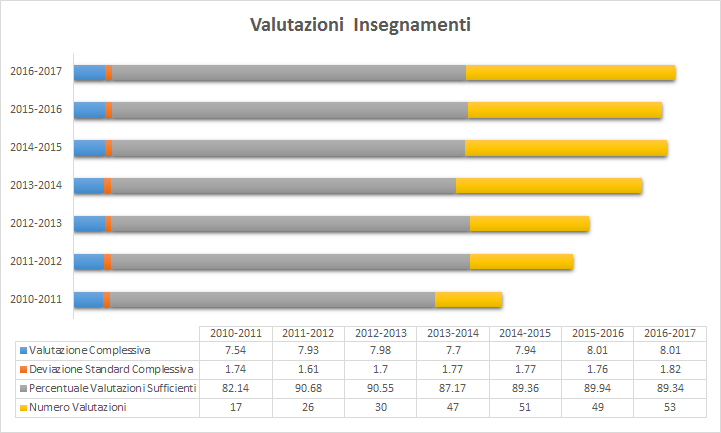
\includegraphics[scale=0.55]{../visual/eval_3.png}
    \end{figure}